\documentclass[a4paper,10pt]{report}

%%%% PRATIQUE POUR LES ALINEAS CHIANTS
\usepackage{indentfirst}

\usepackage[colorlinks=false]{hyperref}

%%%% POUR L'OPTION LABEL= %%%
\usepackage{enumitem}

\setlength{\parindent}{30pt}
\setlength{\parskip}{1ex}
\setlength{\textwidth}{15cm}
\setlength{\textheight}{24cm}
\setlength{\oddsidemargin}{0.2cm}
\setlength{\evensidemargin}{-.7cm}
\setlength{\topmargin}{-.5in}

\usepackage{graphicx}
\usepackage{titling}
\usepackage{listings}
\lstset{%
  basicstyle=\scriptsize\sffamily,%
  commentstyle=\footnotesize\ttfamily,%
  frameround=trBL,
  frame=single,
  breaklines=true,
  showstringspaces=false,
  numbers=left,
  numberstyle=\tiny,
  numbersep=10pt,
  keywordstyle=\bf
}
\newcommand{\subtitle}[1]{%
  \posttitle{%
    \par\end{center}
    \begin{center}\large#1\end{center}
    \vskip0.5em}%
}

%%%%%%%%%%%%%%%% PAGE DE GARDE %%%%%%%%%%%%%%%%%%%%%%
% Crédit : http://www.grappa.univ-lille3.fr/FAQ-LaTeX/6.67.html
\newlength{\larg}
\setlength{\larg}{14.5cm}

%\title{
%{\rule{\larg}{1mm}}\vspace{7mm}
%\begin{tabular}{p{2cm} r}
%   & {\Huge {\bf Méthodes numériques de base}} \\
%   & \\
%   & {\huge Cours de première année - ENSIMAG}
%\end{tabular}\\
%\vspace{2mm}
%{\rule{\larg}{1mm}}
%\vspace{2mm} \\
%\begin{tabular}{p{11cm} r}
%   & {\large \bf } \\
%   & {\large }
%\end{tabular}\\
%\vspace{5.5cm}
%}
%\author{\begin{tabular}{p{13.7cm}}
%    \begin{tabular}{ll}
%        Cours : & Hahmann S.\\
%         & James G.\\
%    \LaTeX : & Poupin P.
%    \end{tabular}
%\end{tabular}\\
%\hline }
\title{OS}
\author{Guillaume Huard \\
	\LaTeX : Poupin Pierre Rouby Thomas
}
\date{}

\begin{document}
\maketitle

%\chapter{Disk Technologies & their impact on OS}

\section{RAID}

Redundant Array of Inexpensive Disks is made of several ordinary disks assembled into one logical larger disk. The objective might be to improve :
\begin{itemize}
  \item performances
  \item reliability
  \item both
\end{itemize}

\subsection{RAID 0}

Also called striping, aims at improving performances.
\begin{figure}[h!]
  \begin{center}
    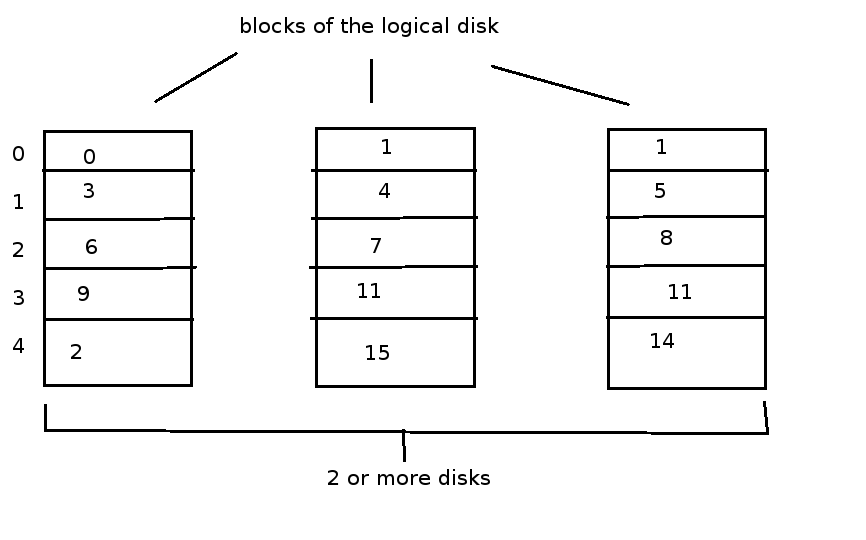
\includegraphics[width=0.8\textwidth]{raid_0.png}
    \caption{}
  \end{center}
\end{figure}

A logical disk in which block n is the block $(n/#disks)$ of disk $(n % #disks)$

Actually the logical disk is divided into chunks which might be larger than the physical block

Also called striping, aims at improving performances.
\begin{figure}[h!]
  \begin{center}
    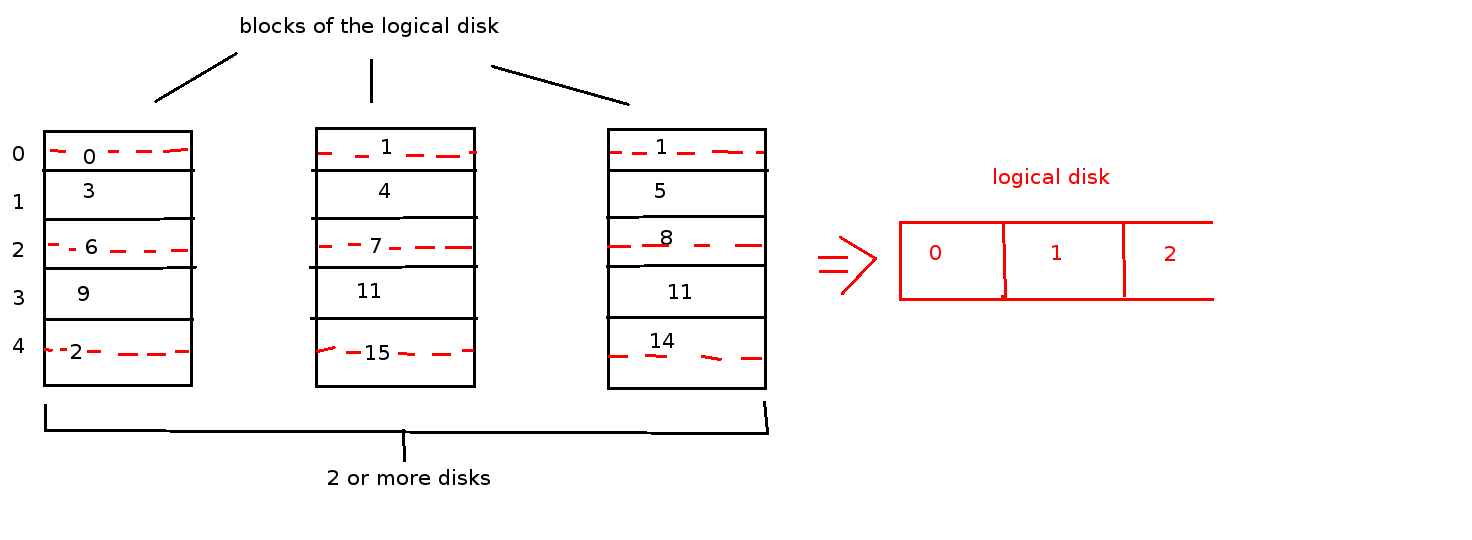
\includegraphics[width=0.8\textwidth]{raid_0_chunks.png}
    \caption{}
  \end{center}
\end{figure}

Advantages :

\begin{itemize}
  \item for large sequential accesses, requests can be issued in parallel on all the disks
  \item some random accesses might be issued in parallel, if they are related to chunks on different disks.
  \item $=>$ Increased Bandwith.
\end{itemize}

Drawbacks :

\begin{itemize}
  \item latency is not improved and might even be degraded
  \item more prone to failure: the probability of failure of the array is larger than the probability of failure of one of the disk
\end{itemize}

\end{document}
